\documentclass{article}

\usepackage[left=2cm,right=2cm, top=2cm, bottom = 2cm]{geometry}
\usepackage{amsfonts}
%%%\usepackage{array}

\usepackage{tikz}

\pagestyle{empty}

%%%\setlength{\tabcolsep}{1.8cm}
%%%\renewcommand{\arraystretch}{2.5}

%%%\makeatletter
%%%\newcommand{\thickhline}{%
%%%    \noalign {\ifnum 0=`}\fi \hrule height 2pt
%%%    \futurelet \reserved@a \@xhline
%%%}
%%%\newcolumntype{!}{@{\hskip\tabcolsep\vrule width 2pt\hskip\tabcolsep}}
%%%\makeatother

\begin{document}

\title{Trigonometric Waveforms}
\date{}

\maketitle

\Large

{\bf \underline{Objective: To understand taking trig functions of any angle}}

{\bf \underline{and the graphs of trig functions.}}

\vspace{5mm}



{\bf Recap of previous material:}

\vspace{5mm}

Consider the right-angled triangle below:

\begin{center}
\begin{tikzpicture}
\draw (0,0) -- (6,0) -- (6,2.5) -- (0,0);
\draw (5.8,0) -- (5.8,0.2) -- (6,0.2);
\node[below] at (3,0) {$12$};
\node[right] at (6,1.25) {$5$};
\draw (1,0) arc (0:22.6:1);
\node[right] at (1,0.3) {$\theta$};
\end{tikzpicture}
\end{center}

\begin{enumerate}
\item Find the length of the hypotenuse.
\item Find $\sin(\theta)$.
\item Find $\cos(\theta)$.
\item Find $\tan(\theta)$.
\item For any angle $\phi$, what equation links $\sin(\phi)$, $\cos(\phi)$, and $\tan(\phi)$?
\item For any angle $\phi$, $1-\sin^2(\phi)=$
\end{enumerate}


\clearpage






{\bf Warm-up:}

\vspace{5mm}

Consider a point in the first quadrant of the plane with coordinates $(a,b)$:

\begin{center}
\begin{tikzpicture}
\draw[->] (-1,0) -- (4,0);
\node[right] at (4,0) {$x$};
\draw[->] (0,-1) -- (0,4);
\node[above] at (0,4) {$y$};
\draw[dashed] (2,0) -- (2,3) -- (0,3);
\draw (0,0) -- (2,3);
\draw[fill] (2,3) circle [radius=0.1];
\node[right] at (2,3) {$(a,b)$};

\node[above left] at (1,1.5) {$r$};
\draw[<->] (0,-0.1) -- (2,-0.1);
\node[below] at (1,0) {$a$};
\draw[<->] (-0.1,0) -- (-0.1,3);
\node[left] at (0,1.5) {$b$};

\draw (1,0) arc (0:56.3:1);
\node[right] at (1,0.5) {$\theta$};
\end{tikzpicture}
\end{center}


\begin{enumerate}
\item Express the length $r$ in terms of $a$ and $b$.
\item Express $a$ in terms of $r$ and $\theta$, using a trigonometric function.
\item Express $b$ in terms of $r$ and $\theta$, using a trigonometric function.
\end{enumerate}

\clearpage


{\bf Theory - Circles and Extending Trigonometric Functions to Arbitrary Angles:}

\vspace{5mm}

We saw above that the distance of a point $(a,b)$ from the origin is $\sqrt{a^2+b^2}$. A circle of radius $r$ consists of all points whose distance from the origin is $r$. Therefore the equation of a circle of radius $r$ centred on the origin is:

\[x^2+y^2=r^2\]

We saw also that:
\[a=r\cos(\theta)\qquad\qquad b=r\sin(\theta)\]
for $\theta$ the angle to the point $(a,b)$ in the first quadrant. We can use this to define $\sin(\theta)$ and $\cos(\theta)$ for any angle $\theta$, even one too large to appear in a right-angled triangle. In a circle of radius 1 centred on the origin, $r=1$, so $\cos(\theta)$ is the $x$-coordinate and $\sin(\theta)$ the $y$-coordinate of the point on the circle at angle $\theta$:

\begin{center}
\begin{tikzpicture}[scale=3]
\draw[->] (-1.5,0) -- (1.5,0);
\node[right] at (1.5,0) {$x$};
\draw[->] (0,-1.5) -- (0,1.5);
\node[above] at (0,1.5) {$y$};

\draw (0,0) circle [radius=1];
\draw[fill] (-0.707,0.707) circle [radius=0.05];
\node[above right] at (0.707,0.707) {$x^2+y^2=1$};

\draw (0,0) -- (-0.707, 0.707);
\node[above left] at (-0.707,0.707) {$(\cos(\theta),\sin(\theta))$};
\draw (0.3,0) arc (0:135:0.3);
\node[right] at (0.2,0.2) {$\theta$};

\draw[dashed] (0,0.707) -- (-0.707,0.707) -- (-0.707,0);
\draw[<->] (-0.707,1.1) -- (0,1.1);
\node[above] at (-0.35,1.1) {$|\cos(\theta)|$};
\draw[<->] (-1.1,0) -- (-1.1,0.707);
\node[left] at (-1.1,0.35) {$|\sin(\theta)|$};
\end{tikzpicture}
\end{center}

See also: \begin{verbatim} https://en.wikipedia.org/wiki/Sine#/media/File:Circle_cos_sin.gif\end{verbatim}

The tangent of an arbitrary angle is then defined by the equation
\[\tan(\theta)=\frac{\sin(\theta)}{\cos(\theta)}\]

\vfill


\clearpage








{\bf Practice:}

\vspace{5mm}

\begin{center}
\begin{tikzpicture}[scale=3]
\draw[->] (-1.5,0) -- (1.5,0);
\node[right] at (1.5,0) {$x$};
\draw[->] (0,-1.5) -- (0,1.5);
\node[above] at (0,1.5) {$y$};

\draw (0,0) circle [radius=1];
\draw[fill] (-0.707,0.707) circle [radius=0.05];
\node[above right] at (0.707,0.707) {$x^2+y^2=1$};

\draw (0,0) -- (-0.707, 0.707);
\node[above left] at (-0.707,0.707) {$(\cos(\theta),\sin(\theta))$};
\draw (0.3,0) arc (0:135:0.3);
\node[right] at (0.2,0.2) {$\theta$};

\draw[dashed] (0,0.707) -- (-0.707,0.707) -- (-0.707,0);
\draw[<->] (-0.707,1.1) -- (0,1.1);
\node[above] at (-0.35,1.1) {$|\cos(\theta)|$};
\draw[<->] (-1.1,0) -- (-1.1,0.707);
\node[left] at (-1.1,0.35) {$|\sin(\theta)|$};
\end{tikzpicture}
\end{center}



\begin{enumerate}
\item In which quadrants of the plane will $\cos(\theta)$ be positive? What ranges of angle does this correspond to?
\item In which quadrants of the plane will $\sin(\theta)$ be positive? What ranges of angles does this correspond to?
\item How are $\sin(\theta)$ and $\sin(-\theta)$ related?
\item How are $\cos(\theta)$ and $\cos(-\theta)$ related?
\item How are $\tan(\theta)$ and $\tan(-\theta)$ related?
\item What is $\tan\left(\frac{\pi}{2}\right)$? Or $\tan\left(\frac{3\pi}{2}\right)$? What about for $\theta$ very near these values?
\end{enumerate}


{\bf Useful Exercise to Try Yourself:}

With some graphing paper (or just draw a grid on some plain paper with a ruler!) and a calculator, draw 3 graphs, one of $\sin(\theta)$, one of $\cos(\theta)$, one of $\tan(\theta)$. Do this by calculating the values of the function to be plotted for several different values of $\theta$, plotting the resulting point, then connecting with a smooth curve. For instance try plotting for $\theta$ taking values between $-7$ and $7$, every $0.5$.

The graphs you should get from this are shown overleaf, with important values of $\theta$ marked.


\clearpage

\begin{center}
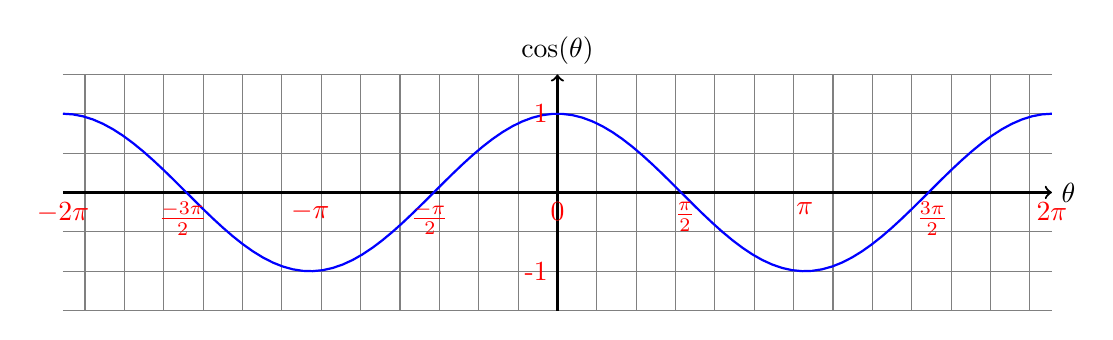
\begin{tikzpicture}
\draw[step=0.5,gray,thin] (-6.28,-1.5) grid (6.28,1.5);
\draw[thick, ->] (0,-1.5) -- (0,1.5);
\node[above] at (0,1.5) {$\cos(\theta)$};
\draw[thick,->] (-6.28,0) -- (6.28,0);
\node[right] at (6.28,0) {$\theta$};

\draw[blue,thick, domain=-6.28:6.28, samples=100] plot (\x,{cos(\x r)});
\node[red,below] at (0,0) {0};
\node[red,below] at (-3.14,0) {$-\pi$};
\node[red,below] at (-1.62,0) {$\frac{-\pi}{2}$};
\node[red,below] at (-4.76,0) {$\frac{-3\pi}{2}$};
\node[red,below] at (-6.28,0) {$-2\pi$};
\node[red,below] at (3.14,0) {$\pi$};
\node[red,below] at (1.62,0) {$\frac{\pi}{2}$};
\node[red,below] at (4.76,0) {$\frac{3\pi}{2}$};
\node[red,below] at (6.28,0) {$2\pi$};
\node[red,left] at (0,1) {1};
\node[red,left] at (0,-1) {-1};
\end{tikzpicture}
\end{center}




\vspace{1cm}




\begin{center}
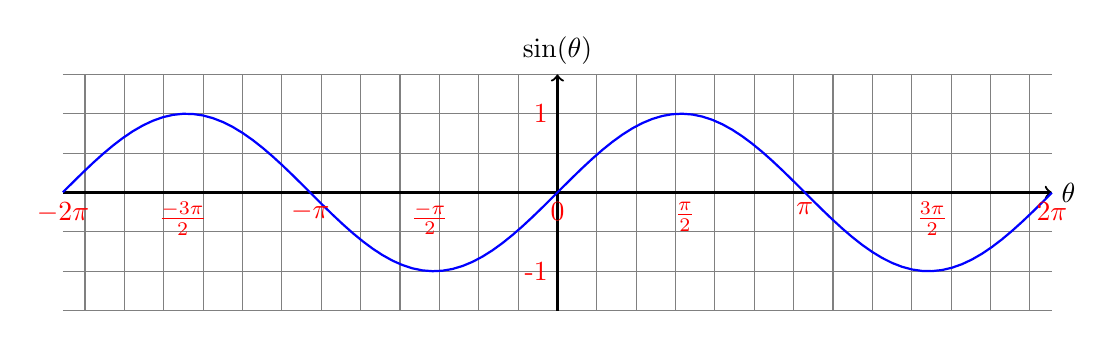
\begin{tikzpicture}
\draw[step=0.5,gray,thin] (-6.28,-1.5) grid (6.28,1.5);
\draw[thick, ->] (0,-1.5) -- (0,1.5);
\node[above] at (0,1.5) {$\sin(\theta)$};
\draw[thick,->] (-6.28,0) -- (6.28,0);
\node[right] at (6.28,0) {$\theta$};

\draw[blue,thick, domain=-6.28:6.28, samples=100] plot (\x,{sin(\x r)});
\node[red,below] at (0,0) {0};
\node[red,below] at (-3.14,0) {$-\pi$};
\node[red,below] at (-1.62,0) {$\frac{-\pi}{2}$};
\node[red,below] at (-4.76,0) {$\frac{-3\pi}{2}$};
\node[red,below] at (-6.28,0) {$-2\pi$};
\node[red,below] at (3.14,0) {$\pi$};
\node[red,below] at (1.62,0) {$\frac{\pi}{2}$};
\node[red,below] at (4.76,0) {$\frac{3\pi}{2}$};
\node[red,below] at (6.28,0) {$2\pi$};
\node[red,left] at (0,1) {1};
\node[red,left] at (0,-1) {-1};
\end{tikzpicture}
\end{center}




\vspace{1cm}




\begin{center}
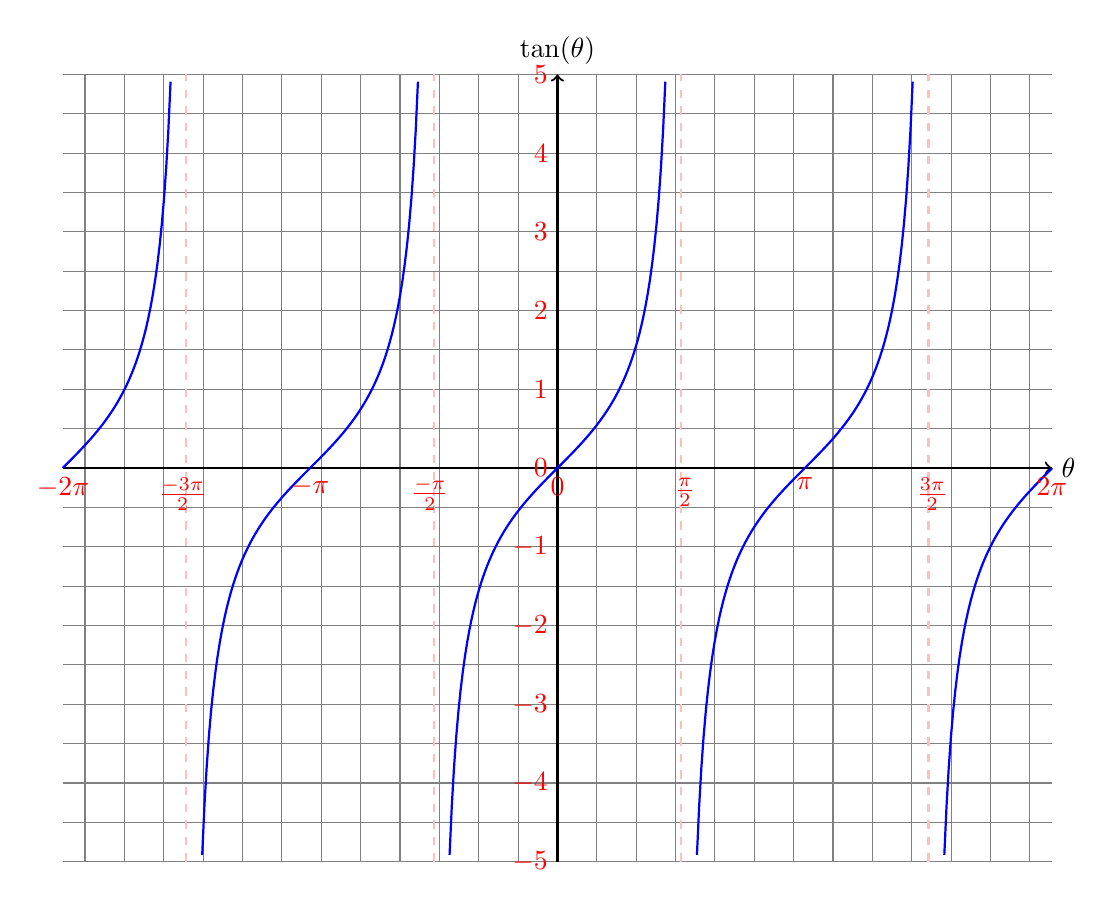
\begin{tikzpicture}
\draw[step=0.5,gray,thin] (-6.28,-5) grid (6.28,5);
\draw[thick, ->] (0,-5) -- (0,5);
\node[above] at (0,5) {$\tan(\theta)$};
\draw[thick,->] (-6.28,0) -- (6.28,0);
\node[right] at (6.28,0) {$\theta$};

\foreach \i in {-1, 0, 1, 2}{
    \pgfmathsetmacro{\start}{\i*pi-1.37}
    \pgfmathsetmacro{\mid}{\i*pi}
    \pgfmathsetmacro{\left}  {(\i-0.5)*pi}
    \draw[dashed, thick,pink] (\left,-5) -- (\left,5); 
    \draw[thick, color=blue] plot [domain=\start:\mid, samples=50] (\x, {tan(\x r)} );
}

\foreach \i in {-2, -1, 0, 1}{
    \pgfmathsetmacro{\mid}{\i*pi}
    \pgfmathsetmacro{\end}  {\i*pi+1.37}
    \draw[thick, color=blue] plot [domain=\mid:\end, samples=50] (\x, {tan(\x r)} );
}


\node[red,below] at (0,0) {0};
\node[red,below] at (-3.14,0) {$-\pi$};
\node[red,below] at (-1.62,0) {$\frac{-\pi}{2}$};
\node[red,below] at (-4.76,0) {$\frac{-3\pi}{2}$};
\node[red,below] at (-6.28,0) {$-2\pi$};
\node[red,below] at (3.14,0) {$\pi$};
\node[red,below] at (1.62,0) {$\frac{\pi}{2}$};
\node[red,below] at (4.76,0) {$\frac{3\pi}{2}$};
\node[red,below] at (6.28,0) {$2\pi$};

\foreach \i in {-5, -4, -3, -2, -1, 0, 1, 2, 3, 4, 5}{
\node[red,left] at (0,\i) {$\i$};
}
\end{tikzpicture}
\end{center}






\clearpage


{\bf Key Points to Remember:}

\vspace{5mm}

\begin{enumerate}
\item The distance from the origin to the point $(x,y)$ is $\sqrt{x^2+y^2}$.
\item The equation of the circle of radius $r$, centred on the origin, is $x^2+y^2=r^2$.
\item For any angle $\theta$, $\cos(\theta)$ (respectively $\sin(\theta)$) is defined to be the $x$-coordinate (respectively, the $y$-coordinate) of the point on the unit circle (radius 1, centre the origin) which makes an angle $\theta$ going anticlockwise from the positive $x$-axis. When $\theta$ is an acute angle, this agree with the right-angled triangle definition.
\item For any angle $\theta$, $\tan(\theta)$ is defined to be $\frac{\sin(\theta)}{\cos(\theta)}$.
\item $\tan(\theta)$ is not defined at angles where $\cos(\theta)=0$; \textit{i.e.}, at $\theta=...\frac{-3\pi}{2}, \frac{-\pi}{2},\frac{\pi}{2},\frac{3\pi}{2},...$.
\end{enumerate}






\end{document}